
% ============================================================
\section{System Design and Architecture}
\label{sec:design}
% ============================================================
% MARKING CRITERION: "System Design and Architecture" [10 marks]
%   - System components clear and well motivated
%   - Overall design of system coherent

\guidance{%
  MARKING: This section is worth 10 marks. The marker will check:
  (1) that each system component is clearly described and its inclusion
  is well motivated, and (2) that the overall design is coherent ---
  i.e.\ the components fit together logically. Include an architecture
  diagram. Explain \emph{why} you chose this design, not just
  \emph{what} it is.}

\subsection{Architecture Overview}

hello \cite{2011Cgp}

\guidance{%
  Provide a high-level overview of the full system. Reference your
  architecture diagram (Figure~\ref{fig:architecture}). Explain how
  data flows through the system from input to output.}

\begin{figure*}[t]
  \centering
  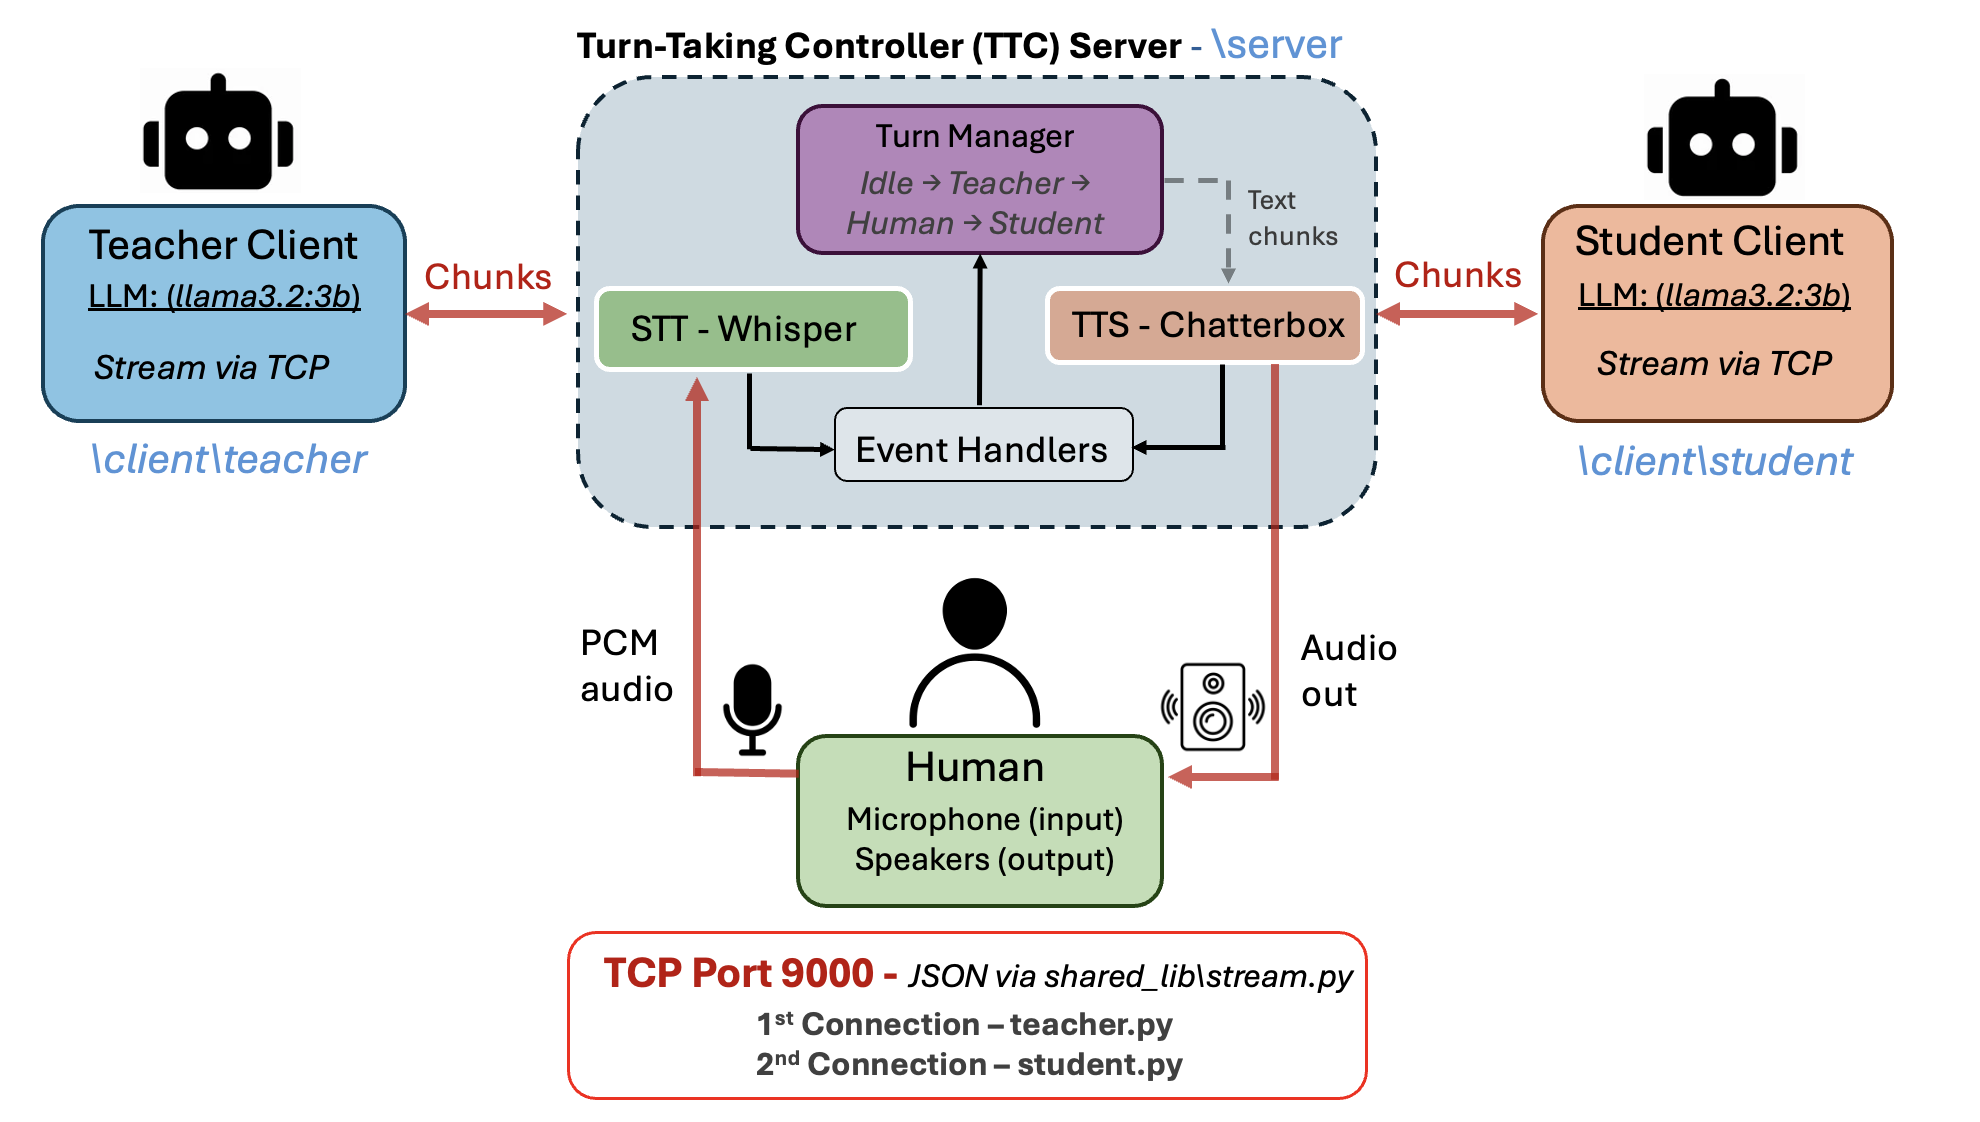
\includegraphics[width=\textwidth]{figures/systemarch.png}
  \caption{Architecture of the proposed system.}
  \label{fig:architecture}
\end{figure*}

\begin{figure*}[t]
  \centering
  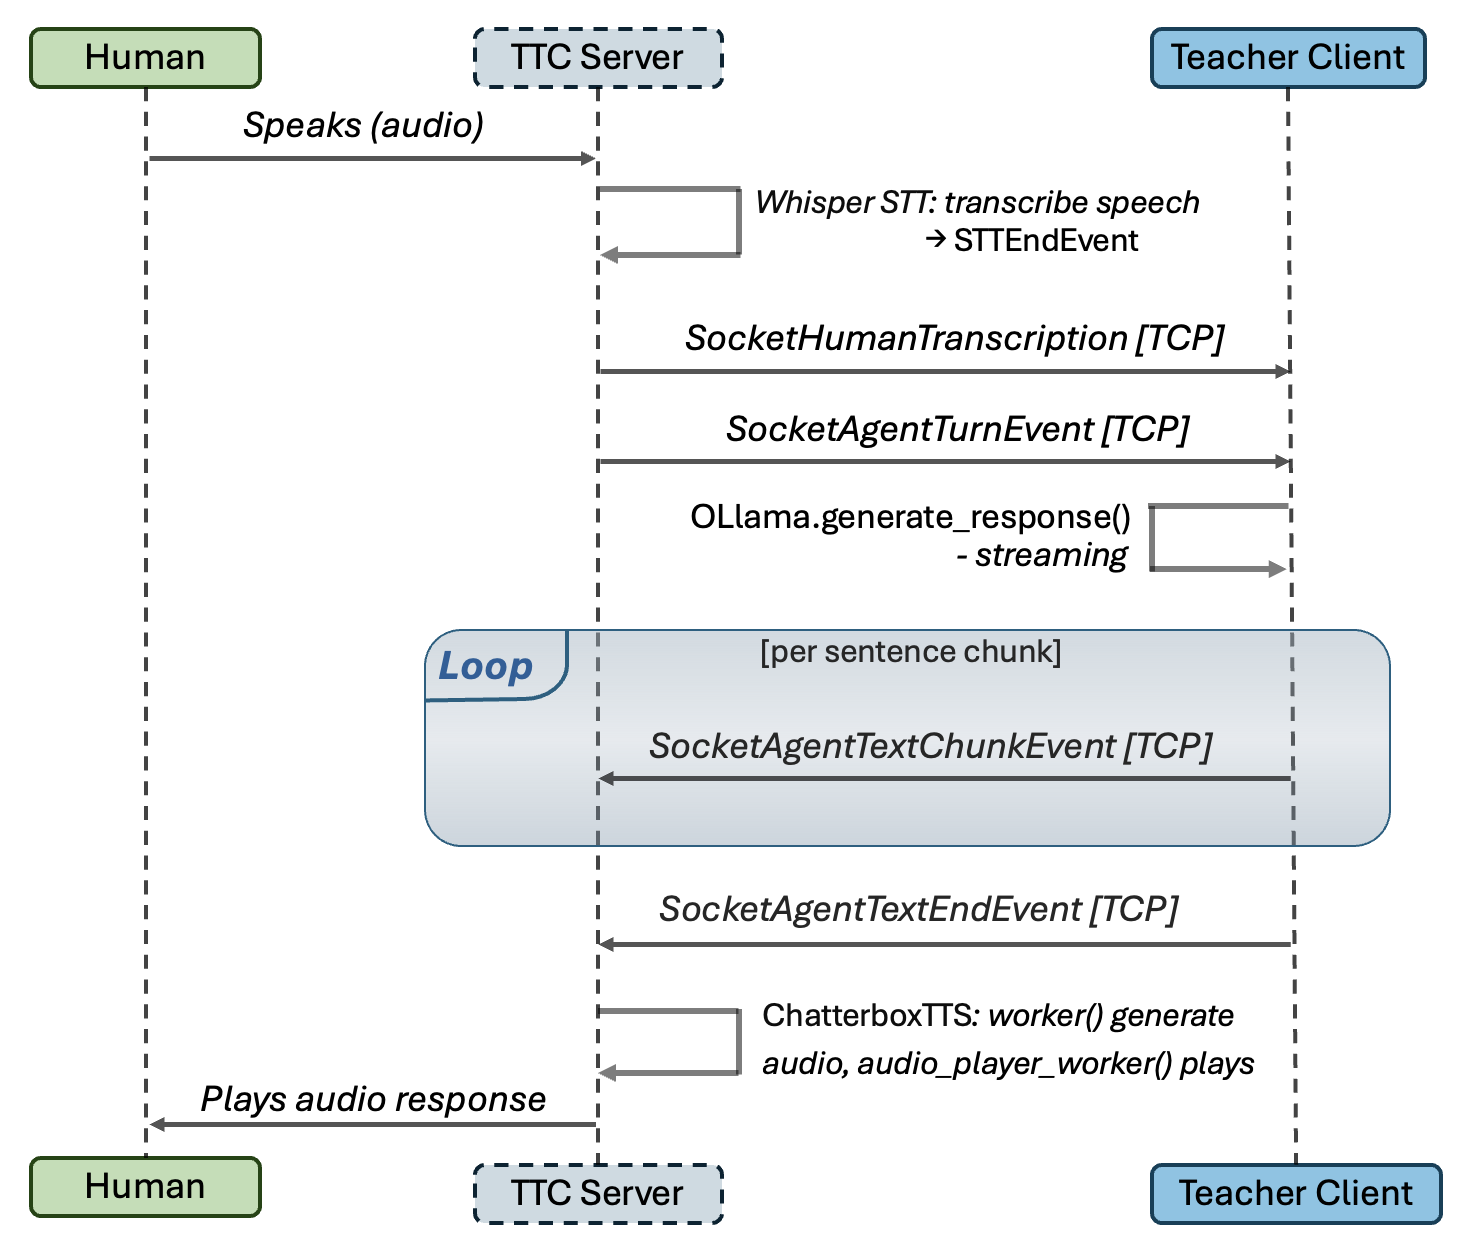
\includegraphics[width=0.72\textwidth]{figures/teacherarch.png}
  \caption{Sequence diagram of the teacher-only interaction workflow (Human, TTC Server, Teacher Client).}
  \label{fig:seq_teacher}
\end{figure*}

\begin{figure*}[t]
  \centering
  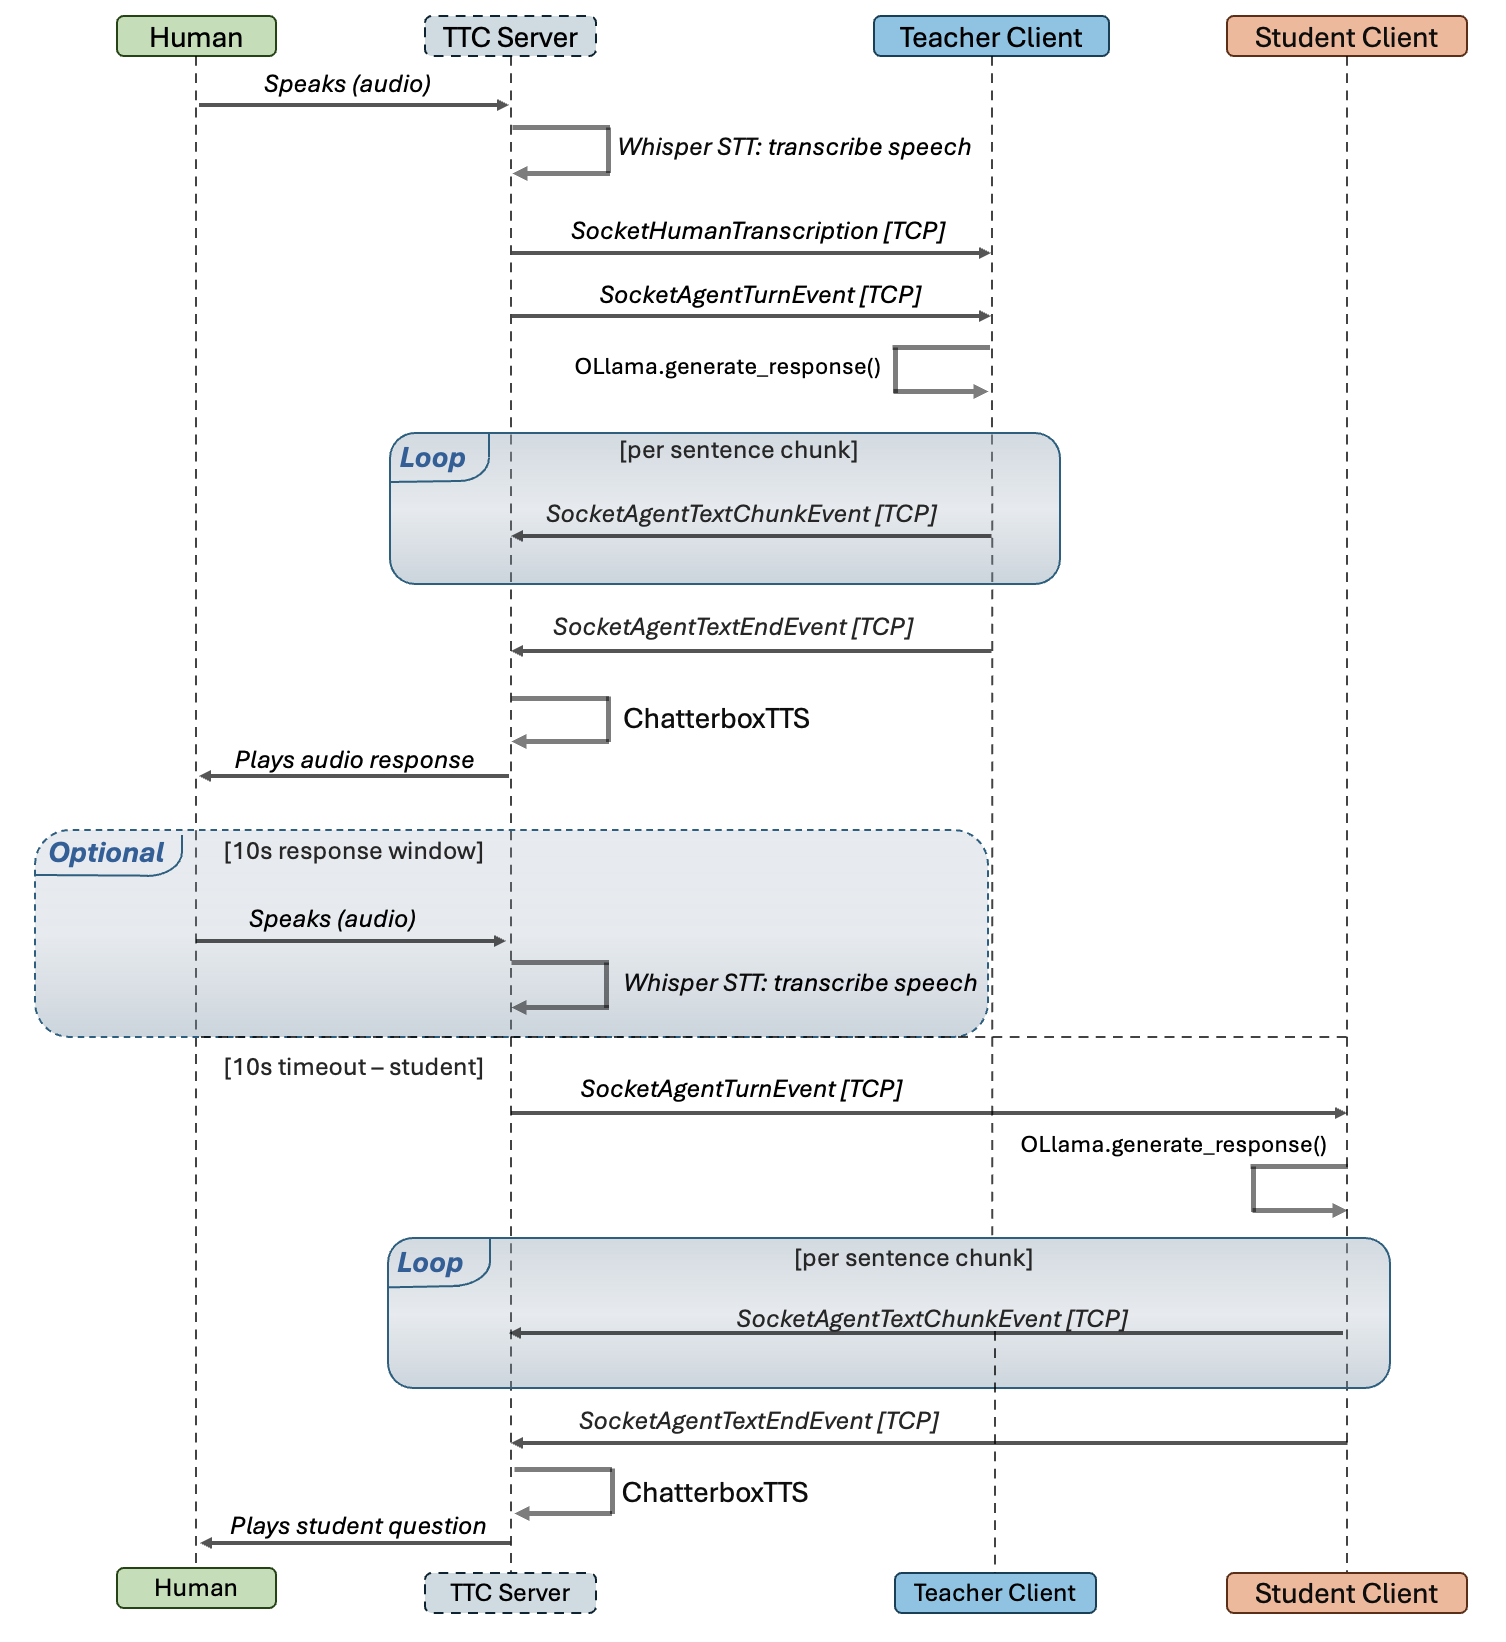
\includegraphics[width=\textwidth]{figures/teacherstudentarch.png}
  \caption{Sequence diagram of the combined teacher--student interaction workflow (Human, TTC Server, Teacher Client, Student Client).}
  \label{fig:seq_combined}
\end{figure*}

% Write architecture overview here.

\subsection{Component A --- [Name]}

\guidance{%
  Describe this component's role in the system, its inputs and outputs,
  and why it was chosen over alternatives. }

% Describe component A.

\subsection{Component B --- [Name]}

% Describe component B.

\subsection{Component C --- [Name]}

% Describe component C (e.g.\ TTS, UI, output module).

\subsection{Design Decisions and Justifications}

\guidance{%
  Summarise the key design trade-offs you made and why. This helps
  demonstrate that the overall design is coherent and well-motivated
  rather than arbitrary.}

% Write design justifications here.

